\subsection{Особенности электронного строения карбонилов d-элементов, описание связи металл – карбонил, включая трехцентровое взаимодействие M-C(O)-M’}							

$$Ni + 4 CO => Ni(CO)_4$$
$$FE + 5 CO => Fe(CO)_5$$


\subsubsection*{Электронное строение}

$CO$ -  лиганд сильного поля, имеющий орбитали, способные к перекрыванию по $\pi$-типу.

\begin{figure}[htp]
\centering
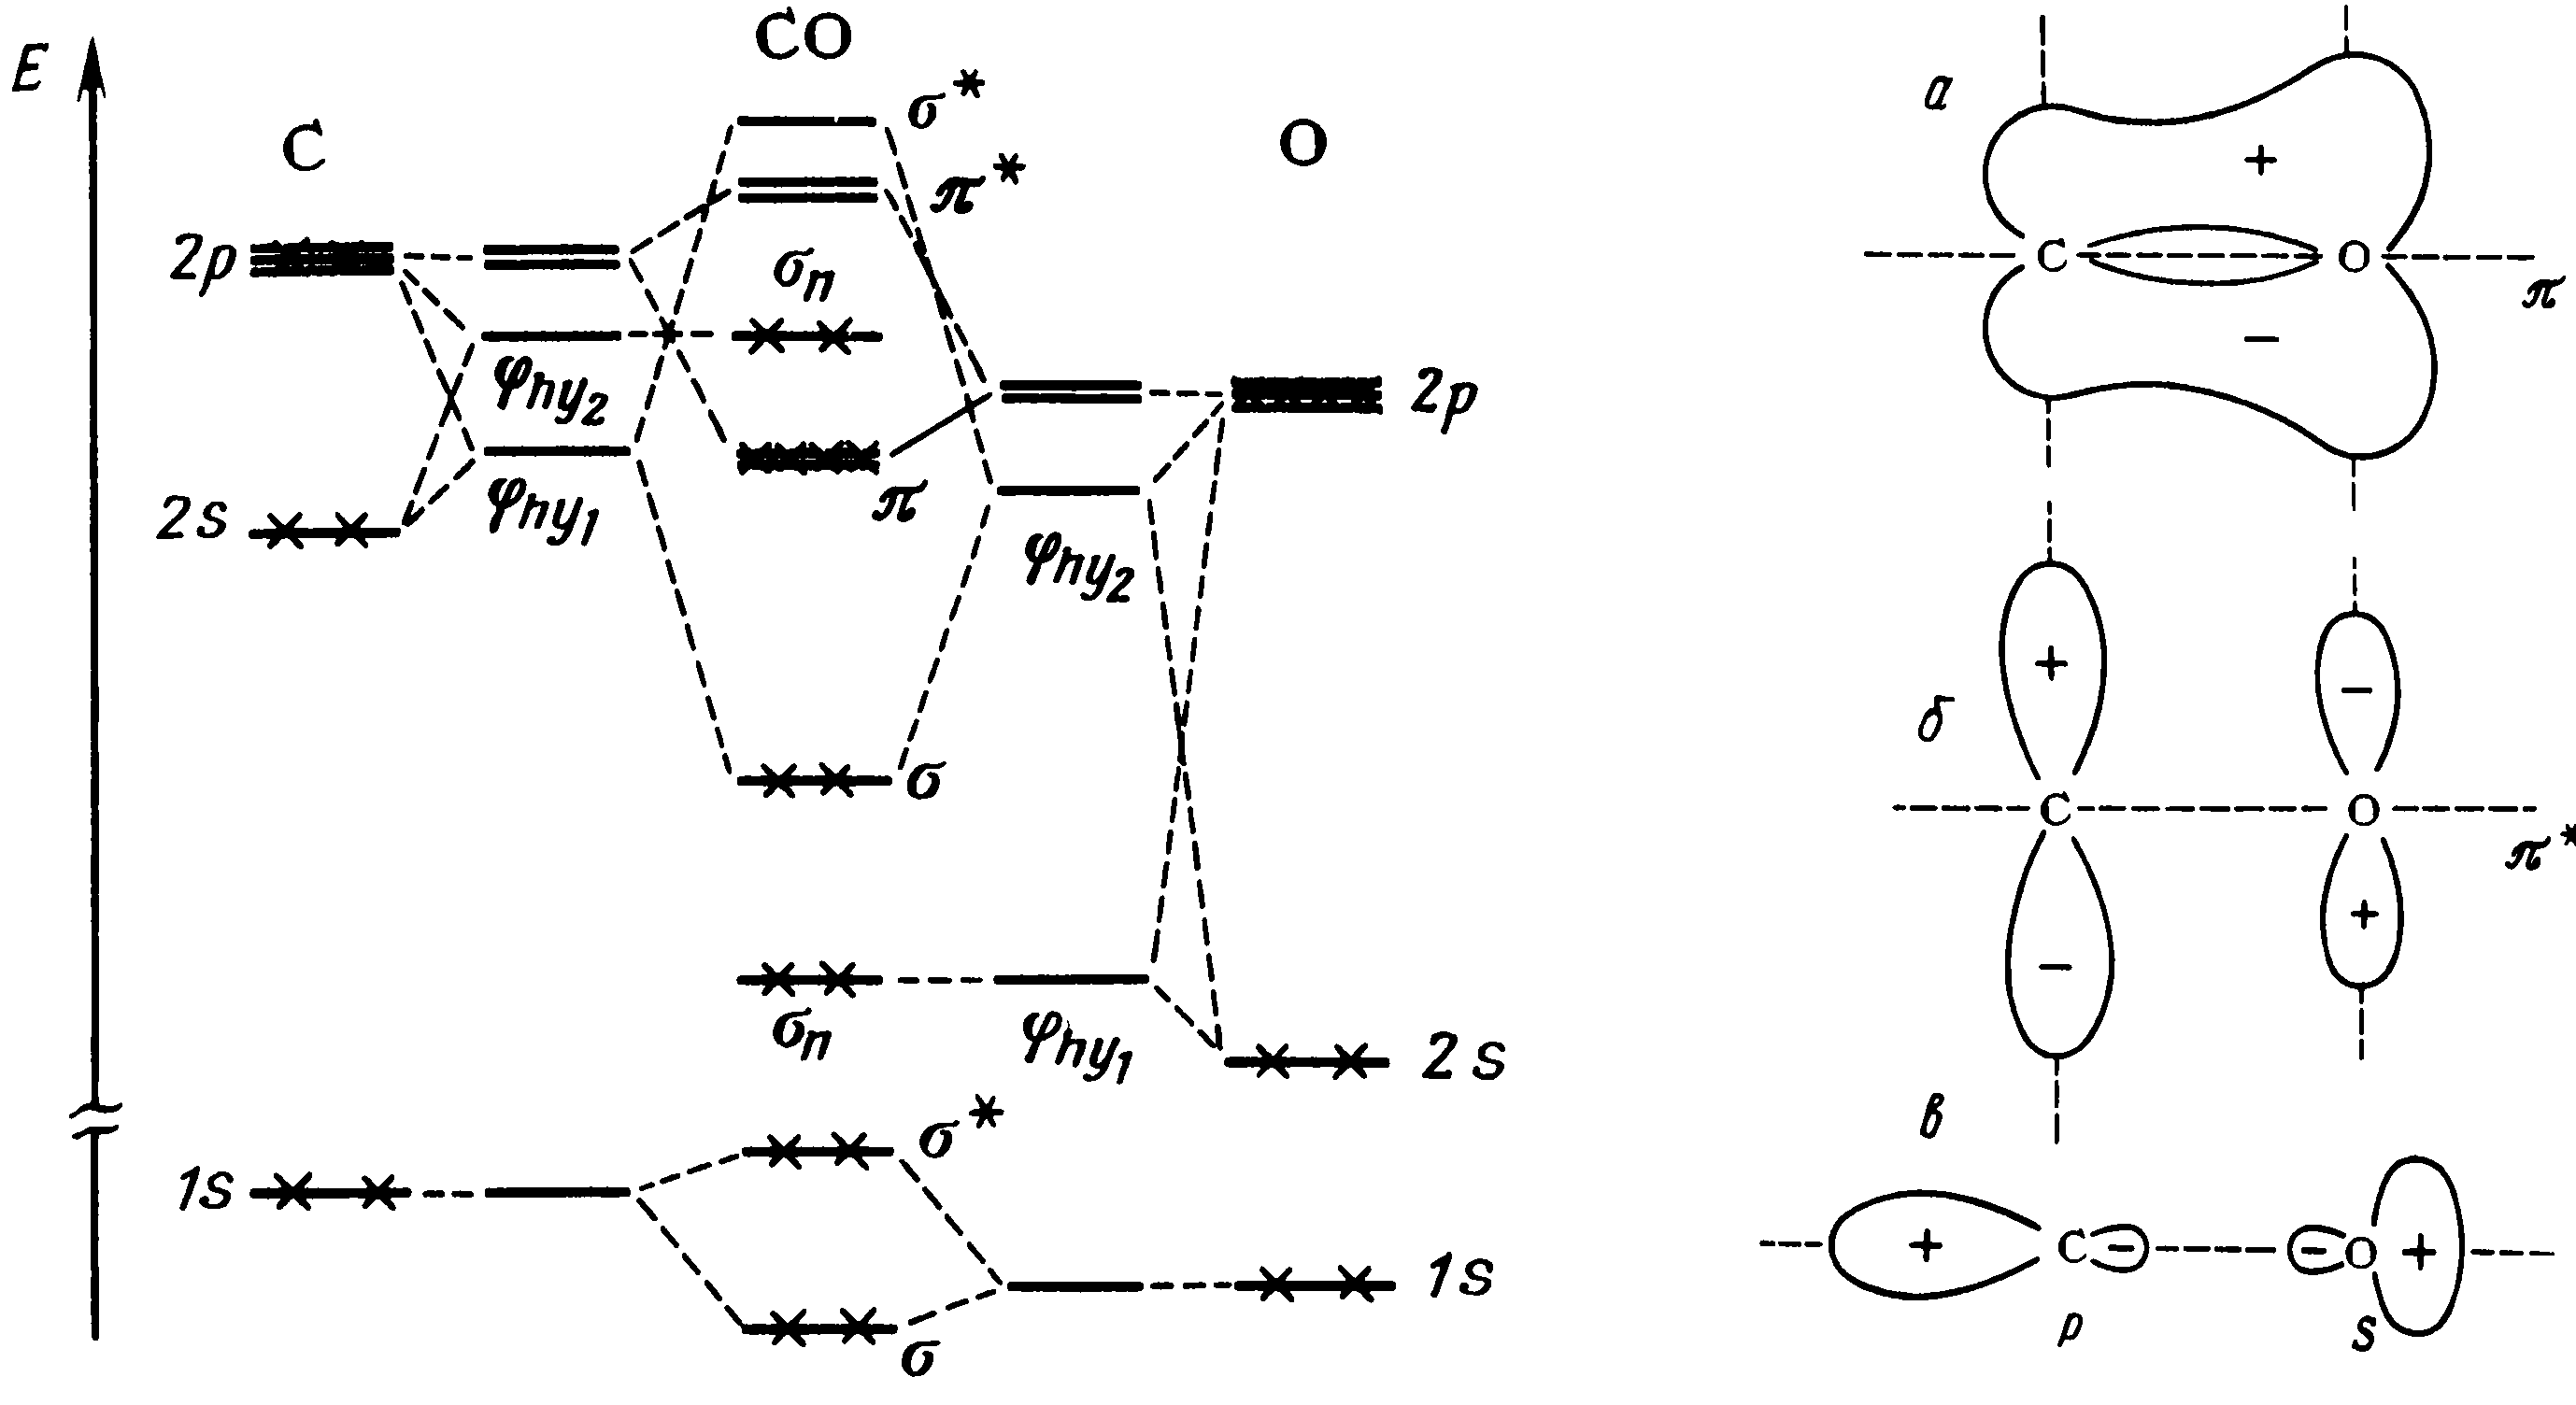
\includegraphics[scale=.800]{images/CO_orbs.png}
\caption{}
\label{}
\end{figure}


\begin{figure}[htp]
\centering
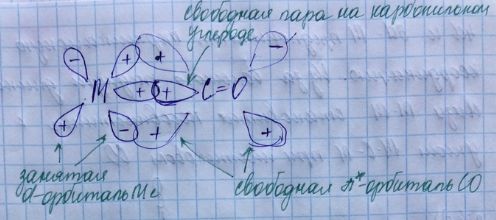
\includegraphics[scale=.800]{images/CO_structure.png}
\caption{}
\label{}
\end{figure}

\begin{itemize}
\item Занятая связывающая орбиталь частично имеет характер $\pi^*-$орбитали карбонила: электронная плотность с металла делокализуется между ним и $CO$, что приводит к удлиннению $CO$ и сокращению порядка связи
\item Это компенсирует донирование на металл неподеленной парой углерода - обратное связывание
\item длинна связи $CO$ в карбонильном лиганде выше, а частота колебаний $CO$ - меньше чем у изолированного $CO$
\end{itemize}

Для металлов в начале характерно насыщение электронной оболочки металла, за счет двухэлектронного донирования.

Для металлов ближе к концу периода d-орбитали заполнены, и металл донирует электроны $CO$















